\mode<presentation>
{
  \usetheme{CambridgeUS}
  \usecolortheme{whale}
  \usecolortheme{lily}

  \setbeamercovered{transparent}
  \usefonttheme[onlymath]{serif}
}

\title[\NyquistStabilityAnalysisShortName] % (optional, use only with long paper titles)
{\course: \NyquistStabilityAnalysisName\license}

\subtitle
{Lecture \NyquistStabilityAnalysisNumber} % (optional)



% If you have a file called "university-logo-filename.xxx", where xxx
% is a graphic format that can be processed by latex or pdflatex,
% resp., then you can add a logo as follows:

%\pgfdeclareimage[height=1.1cm]{university-logo}{UniversityLogo}
%\logo{\pgfuseimage{university-logo}}



% Delete this, if you do not want the table of contents to pop up at
% the beginning of each subsection:
%\AtBeginSection[]
%{
%  \begin{frame}<beamer>{Outline}
%    \tableofcontents[currentsection,currentsubsection]
%  \end{frame}
%}


% If you wish to uncover everything in a step-wise fashion, uncomment
% the following command:

%\beamerdefaultoverlayspecification{<+->}


\begin{document}

\begin{frame}
  \titlepage
\end{frame}

\mode<article>{
\maketitle
\tableofcontents
}

%\mode<presentation>{
%\begin{frame}{Outline}
%  \tableofcontents
%  % You might wish to add the option [pausesections]
%\end{frame}}
\section{More Nyquist Stability Analysis Examples}

\begin{example} Using a Nyquist plot, determine if the following closed loop system is stable
\begin{frame}{Example System}
\begin{center}
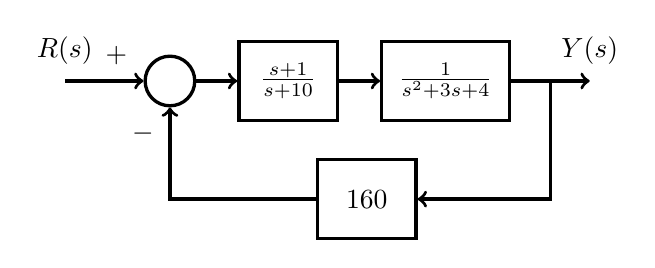
\begin{tikzpicture}[very thick,
sysblock/.style={draw,rectangle,inner sep=6pt,minimum width=1.25cm,minimum height=1.0cm,very thick},
summer/.style={circle,draw,very thick}]

\draw (0,0) node[summer] (sum) {\rule{10pt}{0pt}};
\draw (1.5,0) node[sysblock] (C) {$\frac{s+1}{s+10}$};


\draw (3.5,0) node[sysblock] (G) {$\frac{1}{s^2+3s+4}$};

\draw (2.5,-1.5) node[sysblock] (H) {$160$};

\draw[<-] (sum.180) node[above left=2pt] {$+$} -- ++(-1,0) node[above=2pt] {$R(s)$};
\draw[->] (sum.0) -- (C.180);
\draw[->] (C.0) -- (G.180);
\draw[->] (G.0) -- ++(0.5,0) |- (H.0);
\draw[->] (H.180)  -| (sum.-90) node[below left=2pt] {$-$};
\draw[->] (G.0) ++(0.5,0) -- ++(0.5,0) node[above=2pt] {$Y(s)$};

\end{tikzpicture}
\end{center}
\end{frame}
The loop gain is $L(j\omega) = \frac{(s-10)}{(s-1)(s-2)}$.

First, sketch Bode plot. Although an unstable system does not have a frequency response per se, we can still plot $L(j\omega)$ vs. frequency.
First, factor out the constant terms in $L(s)$:
\[
L(s) = -5\frac{(\frac{s}{-10}+1)}{(\frac{s}{-1}+1)(\frac{s}{-2}+1)}
\]
List the break frequencies
\begin{center}
\begin{tabular}{llll}
\toprule
Break Frequency & Item (P/Z? L/RHP? \#?) & Magnitude Slope & Phase Slope\\\midrule
1 rad/s & 1 RHP pole & -20 dB/dec & 45$^{\circ}$/dec \\
2 rad/s & 1 RHP pole & -20 dB/dec &  45$^{\circ}$/dec \\
10 rad/s & 1 RHP zero & 20 dB/dec & -45$^{\circ}$/dec \\\bottomrule
\end{tabular}
\end{center}

The low frequency term is $-5$, which has a magnitude in dB of $20\log(5) =14$. The magnitude sketch becomes as follows
\begin{frame}{Magnitude Plot}
\begin{center}
\begin{tikzpicture}
\draw (0,0) node {\includegraphics[width=3in]{figures/example1magplot}};
\end{tikzpicture}
\end{center}
\end{frame}

The low frequency term is $-5$, which has a phase of $-180^{\circ}$, which becomes the starting point. We add lines for the regions where each term has a non-zero phase slope, and then follow those directions.
\begin{frame}{Phase Plot}
\begin{center}
\begin{tikzpicture}
\draw (0,0) node {\includegraphics[width=3in]{figures/example1phaseplot}};
\draw[thick,*-*] (-2.15,2.1) -- node[pos=.1,above left] {45$^{\circ}$/dec} ++(3.75,0);
\draw[thick,*-*] (-1.63,2.3) -- node[pos=.1,above] {45$^{\circ}$/dec} ++(3.75,0);
\draw[thick,*-*] (-0.37,2.5) -- node[pos=.2,above] {-45$^{\circ}$/dec} ++(3.75,0);
\end{tikzpicture}
\end{center}
\end{frame}
Now we find the magnitude and phase at an increasing set of frequencies which capture the main characteristics of the frequency response
\begin{frame}{Magnitude and Phase Table}
\begin{center}
\begin{minipage}{2in}
\hspace{-.45in}
\begin{tikzpicture}
\draw (0,0) node {\includegraphics[width=2in]{figures/example1magplot}};
\draw (0,-3) node {\includegraphics[width=2in]{figures/example1phaseplot}};
\end{tikzpicture}
\end{minipage}
\hspace{-.35in}
\begin{minipage}{2.3in}
\begin{tabular}{cccc}
\small Freq (rad/s) & Mag (dB) & Mag & Phase \\\hline
.1 & 14 & 5 & -180$^{\circ}$ \\
.2 & 14 & 5 & -166.5$^{\circ}$ \\
 1  & 14 & 5 & -103.5$^{\circ}$ \\
 2 & 8 & 2.5 & -90$^{\circ}$ \\
 10 & -20 & 0.1 & -58.5$^{\circ}$ \\
100 & -40 &  0.01 & -90$^{\circ}$
\end{tabular}
\end{minipage}
\end{center}
\end{frame}

Draw Nyquist plot.
\begin{frame}{Draw Nyquist Plot}
\begin{center}
\begin{minipage}{2.3in}
\begin{tabular}{cccc}
\small Freq (rad/s) & Mag (dB) & Mag & Phase \\\hline
.1 & 14 & 5 & -180$^{\circ}$ \\
.2 & 14 & 5 & -166.5$^{\circ}$ \\
 1  & 14 & 5 & -103.5$^{\circ}$ \\
 2 & 8 & 2.5 & -90$^{\circ}$ \\
 10 & -20 & 0.1 & -58.5$^{\circ}$ \\
100 & -40 &  0.01 & -90$^{\circ}$
\end{tabular}
\end{minipage}
\begin{minipage}{3in}
\begin{tikzpicture}[scale=.5]
\draw[->] (-8,0) -- (2,0) node[below] {Re$\{s\}$};
\draw[->] (0,-6) -- (0,6) node[left] {Im$\{s\}$};
\draw (-1,-.1) node[below=-3pt] {\small $-1$} -- ++(0,.2);
\draw (-180:5) node[circle,fill,inner sep=0pt,outer sep=0pt,color=green] (a) {\rule{4pt}{0pt}};
\draw (-166.5:5) node[circle,fill,inner sep=0pt,outer sep=0pt,color=cyan] (b) {\rule{4pt}{0pt}};
\draw (-103.5:5) node[circle,fill,inner sep=0pt,outer sep=0pt,color=red] (c) {\rule{4pt}{0pt}};
\draw (-90:2.5) node[circle,fill,inner sep=0pt,outer sep=0pt,color=yellow] (d) {\rule{4pt}{0pt}};
\draw (-58.5:.1) node[circle,fill,inner sep=0pt,outer sep=0pt,color=orange] (e) {\rule{4pt}{0pt}};
\draw (-90:0.01) node[circle,fill,inner sep=0pt,outer sep=0pt,color=purple] (f) {\rule{4pt}{0pt}};
\draw[very thick,color=blue,postaction={decorate,decoration={markings,mark=at position .6 with {\arrow[blue,very thick]{>}}}}] (a)  .. controls ++(-90:.5) and ++(135:.5) .. (b) .. controls ++(-60:.5) and ++(-180:.5) .. (c) .. controls ++(45:1) and ++(-90:1) .. (d) .. controls ++(90:.5) and ++(-90:.5) .. (e) .. controls ++(90:.3) and ++(-180:.3) .. (f);
\draw (-180:5) node[circle,fill,inner sep=0pt,outer sep=0pt,color=green] (aa) {\rule{4pt}{0pt}};
\draw (166.5:5) node[circle,fill,inner sep=0pt,outer sep=0pt,color=cyan] (bb) {\rule{4pt}{0pt}};
\draw (103.5:5) node[circle,fill,inner sep=0pt,outer sep=0pt,color=red] (cc) {\rule{4pt}{0pt}};
\draw (90:2.5) node[circle,fill,inner sep=0pt,outer sep=0pt,color=yellow] (dd) {\rule{4pt}{0pt}};
\draw (58.5:.1) node[circle,fill,inner sep=0pt,outer sep=0pt,color=orange] (ee) {\rule{4pt}{0pt}};
\draw (90:0.01) node[circle,fill,inner sep=0pt,outer sep=0pt,color=purple] (ff) {\rule{4pt}{0pt}};
\draw[very thick,color=blue,postaction={decorate,decoration={markings,mark=at position .6 with {\arrowreversed[blue,very thick]{>}}}}] (aa)  .. controls ++(90:.5) and ++(-135:.5) .. (bb) .. controls ++(60:.5) and ++(180:.5) .. (cc) .. controls ++(-45:1) and ++(90:1) .. (dd) .. controls ++(-90:.5) and ++(90:.5) .. (ee) .. controls ++(-90:.3) and ++(180:.3) .. (ff);
\end{tikzpicture}
\end{minipage}
\end{center}
\end{frame}
Now we can do the Nyquist stability analysis
\begin{itemize}
\item $P=$ \# of unstable poles of $L(s)$. In this case $P=2$.
\item $N=$ \# of clockwise encirclements of $-1+j0$. In this case, we have one counterclockwise encirclement, so $N=-1$.
\item \# of closed loop poles is $Z=N+P = -1+2=1$. Thus, there is one unstable closed loop pole, and the feedback system is not stable.

\end{itemize}


\end{example}\qed

Here is an example for you to try.

\begin{example}
Using a Nyquist plot, determine if the following closed loop system is stable
\begin{frame}{Example System}
\begin{center}
\input{figures/example2blockdiagram.tex}
\end{center}
\end{frame}
\tryit{
\begin{boxedminipage}{6.5 in}
\rule{0pt}{12pt}\vspace{2in}
\color{lightgray}
$P=1, N=-1, Z=-1+1=0$, system is closed loop stable.
\end{boxedminipage}\\
}{\begin{boxedminipage}{6.5in}
\includegraphics[width=5in]{figures/example2soln}
\end{boxedminipage}
}

\end{example}

\section{Nyquist Stability Analysis when $L(s)$ Has Poles on $j\omega$ Axis}

Because the Nyquist plot (so far) was a mapping from the $j\omega$ axis through $L(s)$ back to the complex plane, we run into difficulty whenever $L(s)$ has a pole on the $j\omega$ axis, for in this case $L(j\omega)=\infty$ and we can't plot that big a number.  To cover this situation, we define a modified Nyquist domain that puts a notch to the right around all poles on the $j\omega$ axis, as illustrated below.

\begin{frame}{Modified Nyquist Domain}
\begin{center}
\input{figures/nyquistmappingjwaxis.tex}
\end{center}
\end{frame}

We also need to consider whether to include any poles on the $j\omega$ axis in our count of $P$, since technically these are unstable poles. However, since we are going to notch to the right, around them, these poles will {\em not} be included in the count of $P$.

To draw the Nyquist plot, we fill in all the information for $L(j\omega)$ that we can, and then complete the Nyquist plot by adding the effect of the notches. This is best explained using an example

\begin{example} Using Nyquist stability analysis, determine the stability of the following feedback loop
\begin{frame}
\begin{center}
\input{figures/example3blockdiagram.tex}
\end{center}
\end{frame}

The loop gain $L(s)$ has a pole at $s=0$ and at $s=-2$. Because of the pole at $s=0$, the Nyquist domain must curve around the pole, as shown below. The linear approximation of the Bode plot for $L(s)$ is shown on the right. Note that the magnitude continues to increase as $\omega\rightarrow 0$. This is an effect of that pole at $s=0$. However, for our plot, we only need to start at $\omega=$ a small value, rather than $\omega=0$, 
\begin{frame}
\begin{center}
\begin{minipage}{2in}
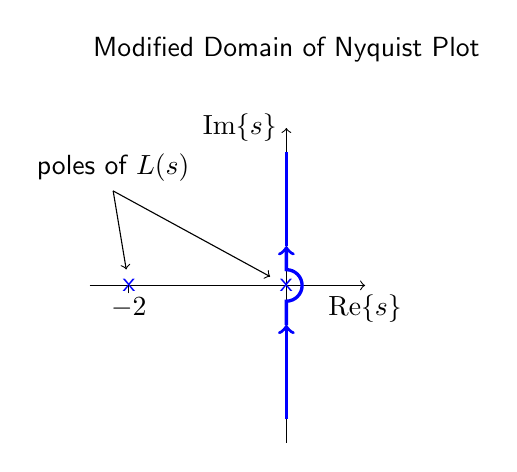
\begin{tikzpicture}[
sysblock/.style={draw,rectangle,inner sep=6pt,minimum width=1.25cm,minimum height=1.0cm,very thick},
summer/.style={circle,draw,very thick}]
\draw (-4,3) node {\textsf{Modified Domain of Nyquist Plot}};
\draw[->] (-4,-2) -- ++(0,4) node[left] {Im$\{s\}$};
\draw[->] (-6.5,0) -- ++(3.5,0) node[below] {Re$\{s\}$};
\draw[->,very thick,color=blue] (-4,-1.7)  -- (-4,-.5); 
\draw[->,very thick,color=blue] (-4,-.5) -- (-4,-0.2) arc (-90:90:.2) -- (-4,.5); 
\draw[very thick,color=blue] (-4,.5) --  (-4,1.7);
\draw (-4,0) node (po1) {\color{blue}\textsf{x}};
\draw (-6,0) node (po2) {\color{blue}\textsf{x}};
\draw (-6,-.1) node[below=-2pt] {$-2$} -- ++(0,.1);
\draw (-6.2,1.5) node (text) {\textsf{poles of $L(s)$}};
\draw[->] (text.-90) -- (po1);
\draw[->] (text.-90) -- (po2);


\end{tikzpicture}
\rule{0pt}{0.8in}
\end{minipage}
\begin{minipage}{2in}\includegraphics[width=2in]{figures/example3magplot}\\
\includegraphics[width=2in]{figures/example3phaseplot}
\end{minipage}
\end{center}
\end{frame}

Let's find the magnitude and phase, starting at $\omega=.1$ and working up.

\begin{frame}{Magnitude and Phase Table}
\begin{center}
\begin{minipage}{2in}
\hspace{-.45in}
\begin{tikzpicture}
\draw (0,0) node {\includegraphics[width=2in]{figures/example3magplot}};
\draw (0,-3) node {\includegraphics[width=2in]{figures/example3phaseplot}};
\end{tikzpicture}
\end{minipage}
\hspace{-.35in}
\begin{minipage}{2.3in}
\begin{tabular}{cccc}
\small Freq (rad/s) & Mag (dB) & Mag & Phase \\\hline
.1 & 26 & 20 & -90$^{\circ}$ \\
.5 & 12 & 4 & -103.5$^{\circ}$ \\
1 & 6 & 2 & -121.5$^{\circ}$ \\
 2  & 0 & 1  & -135$^{\circ}$ \\
  10 & -30 & 0.03 & -166.5$^{\circ}$ \\
 20 & -40 &  0.01 & -180$^{\circ}$
\end{tabular}
\end{minipage}
\end{center}
\end{frame}

This information can be used to build the positive $\omega$ part of the Nyquist plot

\begin{frame}
\begin{center}
\input{figures/example3domain2.tex}
\end{center}
\end{frame}

This is mirrored to create the negative $\omega$ part

\begin{frame}
\begin{center}
\input{figures/example3domain3.tex}
\end{center}
\end{frame}

Contrary to what happened before, the green and cyan dots end up far away on the Nyquist plot on the right, although they start close together on the domain on the left. To complete the Nyquist plot and create a closed curve that can be evaluated, we need to determine how the notch in the Nyquist domain will result as a curve on the Nyquist plot. To figure this out, we examine the magnitude and phase of $L(s)$ part by part. Specifically, recall that
\[
\left|L(s)\right| = \left|\frac{4}{s(s+2)}\right| = \frac{|4|}{|s||s+2|}
\]
and
\[
\angle L(s) = \angle\frac{4}{s(s+2)} = \angle{4} - \angle{s} - \angle (s+2)
\]
Secondly, remember that the magnitude and phase of $s+a$ is determined by the length and angle from horizontal of a line drawn from $a$ to $s$. Thus, to see how $|L(s)|$ and $\angle L(s)$ changes as we go around the notch, we can see how the magnitude and phase of $s$ and $s+2$ change around the notch. In the figure below, we zoom in around the origin, and consider evaluating a particular point $s$ on the notch. We draw a line from the origin to $s$ to represent the term $s$, and a line from $-2$ to $s$ to represent the term $s+2$ or ($s - (-2)$). (In this zoomed-in plot, $-2$ is far to the left, so we don't show the whole line.) 

\begin{frame}
\begin{center}
\begin{tikzpicture}[
sysblock/.style={draw,rectangle,inner sep=6pt,minimum width=1.25cm,minimum height=1.0cm,very thick},
summer/.style={circle,draw,very thick}]
%\draw (-6,3) node {\textsf{Modified Domain of Nyquist Plot}};
\draw[->] (-6,-2) -- ++(0,4) node[left] {Im$\{s\}$};
\draw[->] (-8,0) -- ++(4,0) node[below] {Re$\{s\}$};
\draw[very thick,color=blue,postaction={decorate,decoration={markings,mark=at position .6 with {\arrow[blue,very thick]{>}}}}] (-6,-2)  -- (-6,-1); 
\draw[very thick,color=blue] (-6,-1) arc (-90:90:1) -- (-6,1); 
\draw[very thick,color=blue,postaction={decorate,decoration={markings,mark=at position .6 with {\arrow[blue,very thick]{>}}}}] (-6,1) --  (-6,2);
\draw (-6,0) node (po1) {\Large\color{blue}\textsf{x}};


\draw (-5.293,.707) node[circle,fill,inner sep=0pt,outer sep=0pt,color=blue] (p1) {\rule{4pt}{0pt}} node[right] {$s$};

\draw (-6,0) -- (p1) node[pos=.3,above] {$s$};
\draw (-5.75,0) arc (0:45:.25);
%\draw (-5.5,0) node[above] {$\angle s$};  
\draw (-8,.6) -- (p1) node[pos=.1,above] {$s-(-2)$};
\draw(-10,0) node[right] {$\Leftarrow -2$}; 

\draw (-6,-1) node[circle,fill,inner sep=0pt,outer sep=0pt,color=cyan] {\rule{4pt}{0pt}} node[left] {$-j0.1$};
\draw (-6,1) node[circle,fill,inner sep=0pt,outer sep=0pt,color=green] {\rule{4pt}{0pt}};
%\draw (-6.1,.5) node[left=-2pt] {$0.5j$} -- ++(.2,0) ;
%\draw (-6.1,.-.5) node[left=-2pt] {$-0.5j$} -- ++(.2,0) ;





\end{tikzpicture}
\end{center}
\end{frame}



Now consider two questions
\begin{itemize}
\item How does $|L(s)|$ change as we move along the notch from the cyan dot to the green dot? Answer: very little. Note that $|s|$ doesn't change at all, because the notch is a semicircle. $|s-(-2)|$ changes very little, because the size of the notch is small compared to 2. Thus, when drawing $L(s)$ on the Nyquist plot, we will be moving along a fixed radius, and the curve will either be a circle or a semicircle.
\item How does $\angle L(s)$ change as we move along the notch? Again $\angle s-(-2)$ changes very little from $0^{\circ}$, because the notch is so small. On the other hand, it is easy to see that $\angle s$ goes from $-90^{\circ}$ to $90^{\circ}$ as we move from the cyan dot to the green dot. Thus $\angle s$ changes by $180^{\circ}$. Plugging this into the equation above for $\angle L(s)$, we have that
\[
\Delta \angle L(s) = -180^{\circ}
\]
because of the negative sign in front of $\angle s$.
\end{itemize}
Since a negative angle change corresponds to moving clockwise, this gives us the following rule for drawing the result of the notch:
\begin{center}
\framebox{\begin{minipage}{5in}
When traveling along a notch from below to above (the standard direction of the Nyquist domain), draw a fixed radius curve (semi-circle) in the {\em clockwise} direction, $180^{\circ}$ for every pole in the notch.
\end{minipage}}
\end{center}

Let's apply this rule to complete our example. Using the rule, we start at the cyan dot, and move $180^{\circ}$ clockwise to the green dot to complete the curve.

\begin{frame}
\begin{center}
\input{figures/example3domain5.tex}
\end{center}
\end{frame}

Now for the Nyquist test. Since $L(s)$ has no poles in the right half plane, (remember that poles on the $j\omega$ axis don't count) $P=0$. Since the Nyquist plot does not encircle $-1+j0$, $N=0$. Thus
\[
Z=0+0=0
\]
and the closed loop system has no unstable poles, thus the feedback system is stable.

\end{example}\qed

\section{Lecture Highlights}
The primary takeaways from this article include
\begin{enumerate}
\setlength{\itemsep}{5pt}
\setlength{\parskip}{0pt}
\setlength{\parsep}{0pt}
\item This article gives additional examples of determining closed loop stability using the Nyquist plot. Please see the Lecture Highlights from the previous lecture article for big picture highlights about Nyquist.
\item Drawing a Nyquist plot for systems with open loop poles on the imaginary axis requires special care, as shown in this lecture's examples.
\end{enumerate}


\section{Quiz Yourself}

\subsection{Questions}

\begin{enumerate}
\setlength{\itemsep}{5pt}
\setlength{\parskip}{0pt}
\setlength{\parsep}{0pt}
\item Consider the following feedback control system
\begin{center}
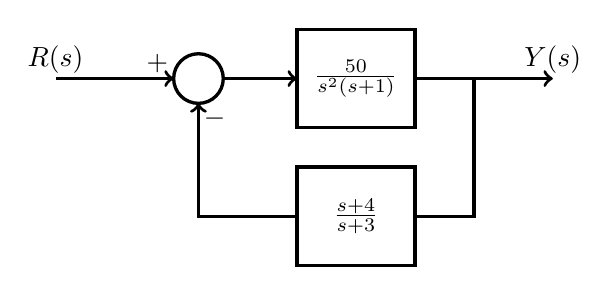
\begin{tikzpicture}[scale=1,inner sep=0pt,outer sep=0pt,very thick,
sysblock/.style={draw,rectangle,inner sep=2pt,minimum width=1.5cm,minimum height=1.25cm,very thick}]
\draw (5,0) node[draw,circle] (sum3) {$\rule{0pt}{18pt}$};
%\draw (7,0) node[draw,circle] (sum2) {$\rule{0pt}{18pt}$};
\draw (7,0) node[sysblock] (G) {$\frac{50}{s^{2}(s+1)}$};
\draw (7,-1.75) node[sysblock] (Kd) {$\frac{s+4}{s+3}$};

\draw[<-] (sum3.180)  node[above left=2pt] {$+$} -- ++(-1.5,0) node[above=2pt] {$R(s)$};
\draw[->] (sum3.0) -- (G);
\draw[->] (G) -- ++(2.5,0) node[above=2pt] {$Y(s)$};
\draw[->] (G) ++(1.5,0) |- (Kd) -| (sum3.-90) node[below right=2pt] {$-$};
%\draw[<-] (sum2.90) node[above right=2pt] {$+$} -- ++(0,1) node[right=2pt] {$D(s)$};
\end{tikzpicture}
\end{center}
Sketch the Bode plot of the loop gain $\frac{50}{s^{2}(s+1)}\frac{s+4}{s+3}$, and using the information from this plot, sketch the Nyquist plot. Determine if the closed loop system is stable or unstable.
\item Consider the following feedback control system
\begin{center}
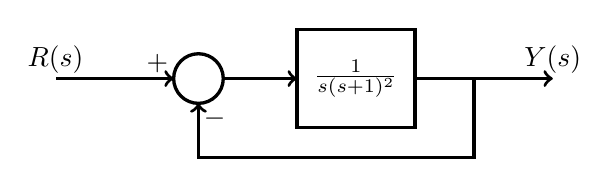
\begin{tikzpicture}[scale=1,inner sep=0pt,outer sep=0pt,very thick,
sysblock/.style={draw,rectangle,inner sep=2pt,minimum width=1.5cm,minimum height=1.25cm,very thick}]
\draw (5,0) node[draw,circle] (sum3) {$\rule{0pt}{18pt}$};
%\draw (7,0) node[draw,circle] (sum2) {$\rule{0pt}{18pt}$};
\draw (7,0) node[sysblock] (G) {$\frac{1}{s(s+1)^2}$};

\draw[<-] (sum3.180)  node[above left=2pt] {$+$} -- ++(-1.5,0) node[above=2pt] {$R(s)$};
\draw[->] (sum3.0) -- (G);
\draw[->] (G) -- ++(2.5,0) node[above=2pt] {$Y(s)$};
\draw[->] (G) ++(1.5,0) -- ++(0,-1)  -| (sum3.-90) node[below right=2pt] {$-$};
\end{tikzpicture}
\end{center}
Use \textsc{Matlab} to plot the Bode plot for $G(s)$. Using this, sketch the Nyquist plot. Determine if the closed loop system is stable or unstable.
\end{enumerate}


\subsection{Solutions}
\begin{enumerate}
\setlength{\itemsep}{5pt}
\setlength{\parskip}{0pt}
\setlength{\parsep}{0pt}
\item \rule{12pt}{0pt}
\begin{center}
\includegraphics[width=6in]{quizfigures/1asoln}\\
\includegraphics[width=6in]{quizfigures/1bsoln}
\end{center}
\newpage
\item \rule{12pt}{0pt}
\begin{center}
\includegraphics[width=5in]{quizfigures/2asoln}\\
\includegraphics[width=5in]{quizfigures/2bsoln}
\end{center}
\end{enumerate}


\end{document}
